\section{Pose Graph Optimization}

When the amount of registered captures increment, the accumulated error 
becomes more visible. There is a drift respect to the real sensor trajectory. 
In order to afront this problem the most common approach is to use a pose graph 
optimization algorithm. 

Each pose of the sensor (4x4 Transformation Matrix) represents a node of the 
graph and each restriction between two poses represents an edge. The relative 
transformation between the two poses is used as restriction and it is possible 
to add different kinds of restrictions if more information is available.

Then we have a least squares minimization problem that can be described by the following equation:

$$ F(x) = \sum\limits_{<i,j> \in C } e(x_i,x_j,z_{ij})^T \Omega_{ij} e(x_i,x_j,z_{ij}) $$

$$ x^* = \mathop{\rm argmin}_x F(x) $$

Where $x=\{x_1,x_2,...,x_n\}$ and each $x_i$ represents a parameter block , $z_{i,j}$ and $\Omega_{ij}$ represents the mean  
 and the information matrix  of a constraint 
relating parameters $x_i$ and $x_j$.

In our case $x_i$ is the 4x4 transformation matrix, corresponding to a sensor pose. $z_{i,j}$ is the 
relative transformation between the pose $x_i$ and the pose $x_j$ and $\Omega_{ij}$ is the weight or 
the confidence we give to the restriction.

the $e_{ij}$ is defined as follows:

$$
e(x_i,x_j,z_{ij}) = z_{ij} - \hat{z_{ij}}
$$

Where $\hat{z_{ij}}$ is the relative transformation obtained directly from the pose graph and $\hat{z_{ij}}$ 
is the relative transformation calculated applying the proposed ICP to the i-esim capture and j-esim capture.


To simplify notation let 

$$
e(x_i,x_j,z_{ij}) = e(x_i,x_j) = e_{ij}(x)
$$

\begin{equation}
\label{eq:errorAprox}
e_{ij}(x + \Delta x) \simeq e_{ij}(x) + J_{ij} \Delta x
\end{equation}


\begin{equation}
\label{eq:globalFunc}
F_{ij}(x + \Delta x) = e_{ij}(x + \Delta x)^T \Omega_{ij}  e_{ij}(x + \Delta x)
\end{equation}

\begin{equation}
\label{eq:globalFuncAprox}
F_{ij}(x + \Delta x) \simeq (e_{ij}(x) + J_{ij} \Delta x)^T \Omega_{ij}  (e_{ij}(x) + J_{ij} \Delta x)
\end{equation}

\begin{equation}
\label{eq:globalFuncAprox2}
 =  \underbrace{e_{ij}(x)^T \Omega_{ij} e_{ij}(x)}_{c_{ij}} + 2  \underbrace{e_{ij}(x)^T \Omega_{ij} J_{ij}}_{b_{ij}} \Delta x + \Delta x^T \underbrace{ J_{ij}^T  \Omega_{ij} J_{ij}}_{H_{ij}} \Delta x
\end{equation}

\begin{equation}
\label{eq:globalFuncAprox2}
 = c_{ij} + 2 b_{ij} \Delta x + \Delta x^T H_{ij} \Delta x
\end{equation}

This is a non linear least squares problem and can be solved using 
methods such as for example Gauss-Newton or Levenber-Marquardt.





G2o is a library that contains non linear error functions optimization 
algorithms for graphs and is widely used in registration algorithms. 

The poses where optimized using this library and specifically the 
Levenber-Marquardt algorithm.



\subsection{Loop Closure}

When the sensor vists the same region at different times, for example following 
a circular trajectory. A restriction between two non-consecutive captures can be 
added to the graph. In the case of a circular trajectory, the accumulated error 
is very noticeable when the initial and the final capture are connected. If a 
restriction between this two captures is added to the graph it is possible to 
adjust the position of all poses in order to satisfy the restriction. This 
is called Loop Closure.



\subsection{Loop Detection}

In order to detect previously visited areas of the scene SURF \cite{Bay06surf} feature detector 
is used. This algorithm finds image corners, looking for strong responses in two ortogonal directions. 


$$
H = \begin{bmatrix} I_{xx} & I_x I_y \\ I_x I_y & I_{yy} \end{bmatrix} \begin{bmatrix} u \\ v \end{bmatrix}
$$

$$
det(H) = I_{xx} I_{yy} - I_{xy}^2;
$$


The second order partial derivatives are approximated using just a box filter, in other words 
summing and substracting pixel values without using gaussian weighing. When extracting features 
usually the image is scalled (scale-space) to different sizes in order to find image structures 
at different scales. SURF algorithm instead of scale the image, scales the filter applied to the 
image, increasing the speed of the calculations in one order of magnitude.


\begin{figure}
\begin{center}
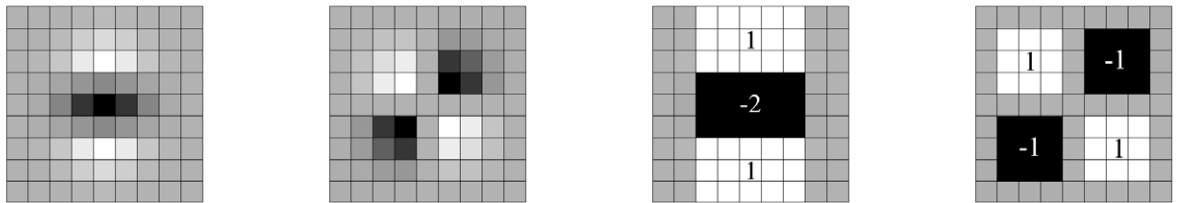
\includegraphics[scale=0.35]{images/surf_mask}
\caption{Left to right: the (discretised and cropped) Gaussian second order partial derivatives 
in y-direction and xy-direction, and approximations using box filters. 
Grey regions are equal to zero. Image extracted from \cite{Bay06surf}}
\end{center}
\end{figure}

